\documentclass[11pt]{amsart}
\usepackage[T1]{fontenc}
\usepackage[utf8]{inputenc}
\usepackage{amsmath,amssymb,amsthm}
\usepackage{array}
\usepackage{booktabs}
\usepackage{graphicx}
\usepackage{geometry}
\usepackage{xcolor}
\usepackage{hyperref}
\usepackage{enumitem}
\geometry{margin=1in}
\setlength{\emergencystretch}{3em}
\graphicspath{{../foundations_v2/figures/}}
\hypersetup{colorlinks=true,linkcolor=blue!50!black,citecolor=blue!50!black,urlcolor=blue!50!black,pdftitle={SEION Math Core: A Reproducible Verification Suite},pdfauthor={Eliuth Chavero Jasso}}

\title[SEION Math Core reproducibility companion]{SEION Math Core: A Reproducible Verification Suite for Finite-Dimensional N-Ary Algebra}
\author{Eliuth Chavero Jasso}
\address{Independent Researcher, Apizaco, Tlaxcala, Mexico}
\thanks{Verified email and ORCID metadata remain a repository blocker.}
\date{Research v2 companion, 29 July 2026}

\begin{document}
\begin{abstract}
This companion documents the software and artifact protocol for the finite-dimensional structure-preserving reduction experiments in the associated foundations draft. It separates a coordinate-loop reference implementation from vectorized NumPy contractions, records dense and CP law representations, and registers every run with source, configuration, mathematical-object, and input-artifact hashes. The current matrix contains 180 complete rows, five seeds for each principal family, exact assumption-removal counterexamples, dense/CP rank controls, positive-gap and no-gap spectral controls, and CPU/GPU parity records. The companion makes no mathematical novelty claim and does not convert reproducibility infrastructure into a theorem.
\end{abstract}
\maketitle

\section{Scope}

The software track is deliberately independent of the foundations claim. It
answers a narrower question: can a reader regenerate the finite tensors,
reduction residuals, bounds, figures, tables, and parity checks from one
repository command? The answer is yes for the current local environment,
subject to the missing-author-metadata blocker and the scientific novelty
blocker recorded in the foundations draft.

\section{Repository architecture}

\begin{center}
\small
\begin{tabular}{p{.55\textwidth}>{\raggedright\arraybackslash}p{.30\textwidth}}
\toprule
path & role\\
\midrule
\url{src/seion_core/research_v2/reference.py} & coordinate-loop evaluator\\
\url{src/seion_core/research_v2/accelerated.py} & Einstein/tensordot evaluator\\
\url{tests/research_v2/} & parity, theorem-example, and counterexample tests\\
\url{experiments/matrices/research_v2_matrix.yaml} & resolved experiment families\\
\url{artifacts/runs_v2/} & immutable-style per-run manifests and inputs\\
\url{artifacts/index/*_v2.*} & derived indexes and summaries\\
\url{papers/foundations_v2/figures/} & vector PDF/SVG figure suite\\
\bottomrule
\end{tabular}
\end{center}

\section{Artifact contract}

Each run has a stable run identifier derived from
\[
\begin{gathered}
(\text{experiment},\text{configuration hash},\text{object hash},\\
\text{input hash},\text{seed},\text{precision},\text{backend},\\
\text{device},\text{implementation version})
\end{gathered}
\]
The manifest also records the source commit and whether the worktree was
dirty. Numerical rows include runtime, peak traced RAM, VRAM when available,
convergence status, and failure count. Historical artifacts under
\texttt{artifacts/runs/} are not overwritten.

\section{Parity protocol}

The reference evaluator performs explicit coordinate summation. The
accelerated evaluator uses independently ordered contractions. Tests compare
real and complex laws of arity \(2,3,4\), all ternary partial-composition
slots, and repeated-leaf trees. The theorem-example tests additionally check
exact reduction on a rational block-supported tensor, the approximate tree
bound, and both assumption-removal counterexamples.

\begin{figure}[t]
\centering
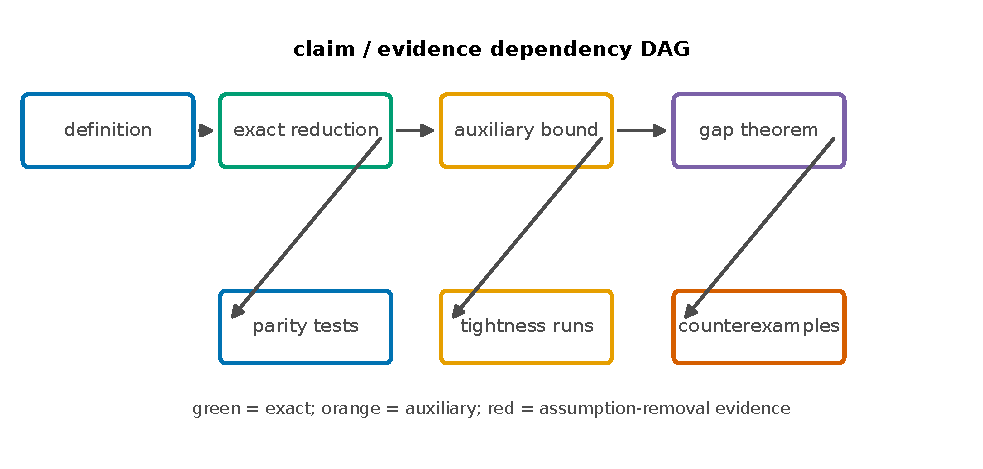
\includegraphics[width=.82\textwidth]{fig09_claim_evidence_dag}
\caption{Claim/evidence dependency graph used by the v2 release audit.}
\end{figure}

\section{Experiment matrix}

The principal families are:
\begin{enumerate}[leftmargin=*]
\item approximate-closure tree errors at four residual levels and three tree
families;
\item known, random, PCA, SVD, spectral, and closure-minimizing projectors;
\item exact dense and CP rank-sweep representations;
\item positive-gap threshold snapping and a no-gap rank-flip control;
\item CPU/GPU contraction parity when CUDA is available.
\end{enumerate}

The generated summary reports mean, standard deviation, median, extrema, a
normal-approximation 95 percent confidence half-width, effect size versus the
registered reference when defined, runtime, memory, convergence, and
failures. Repeated historical rows are not treated as scientific replicates.

\section{Figures and tables}

The nine v2 figures are generated as PDF and SVG from registered CSV rows.
Quantitative plots carry uncertainty and theoretical reference bounds; the
conceptual diagrams are explicitly labeled as definitions or dependency
graphs. Tables use booktabs-style LaTeX output generated from the same
indexes. No categorical dtype sequence is plotted as a continuous variable.

\section{Reproduction and release gate}

The exact commands are in \texttt{papers/software\_v2/README.md}. The local
run produced 180 complete rows, 100 unique object/input/seed experiment keys,
and five CPU/GPU parity records. The strict gate remains red/yellow until a
genuinely new mathematical result and verified author metadata are supplied.
This is consistent with reproducibility guidance that code, data, and
parameter settings must be sufficient to regenerate tables and figures
\cite{SISCInstructions}.

\section{Conclusion}

SEION Math Core v2 now separates proof objects, reference computation,
accelerated computation, registered evidence, and publication output. The
companion is a software and reproducibility report; it does not substitute
for the mathematical novelty that the foundations manuscript still lacks.

\bibliographystyle{amsplain}
\bibliography{references}
\end{document}
